\documentclass{article}
\usepackage{amsmath}
\usepackage{natbib}
\usepackage{graphicx}
\usepackage{subfig}
\usepackage{bm}
\usepackage{appendix}
\usepackage{authblk}

% Special commands 
\newcommand{\vect}[1]{\boldsymbol{\mathbf{#1}}}
\providecommand{\e}[1]{\ensuremath{\times 10^{#1}}}

\title{Domestic Trade and Inequality}
\author[1]{Farid Farrokhi}
\author[2]{David Jinkins\thanks{We thank Sina Smid for research assistance, and participants in seminars at Copenhagen Business School and Cardiff University for helpful suggestions.}}
\affil[1]{Penn State}
\affil[2]{Copenhagen Business School}
\renewcommand\Authands{ and }

\begin{document}
\maketitle

Inequality has long fascinated economists, and growing income inequality has been heatedly discussed in public forums recently.\footnote{It is not every year that a 700-page collection of charts and academic theory on inequality is a New York Times bestseller.}  In this paper, we add to this discussion by documenting some new facts about the interaction of geography with inequality, and developing a model which can rationalize what we find.  After estimating the model on American data, we will discuss the effect of changes in geography on inequality.  These changes might be a new highway, or population movement due to climate change.

Our first empirical contribution is to document facts about inequality and geography.  We assign to each American city a measure of remoteness meant to capture its distance from all other cities.  We then show that this measure correlates negatively with the skill premium, the ratio of the mean wage of the highly educated to the mean wage of the less educated.  That is, highly educated workers make less relative to less educated workers in remote cities.  On the other hand, conditional on population and other controls, the more remote a city is, the higher its share of highly educated workers, which we call the college share.  As far as we know, our paper is the first to document these facts.

At least since the development of new economic geography, economists have examined the role of trade costs in determining the location of manufacturing centers \textbf{CITE KRUGMAN,allen arkolakis}.  On the other hand, recent models of spatial inequality have treated cities as isolated.  Workers in a city can interact with each other, but there is no interaction between cities.  This literature, then, has no way to discuss the interaction of geography with inequality, since the geographic location of a city relative to other cities is irrelevant.  By including intra-city trade in an model of inequality, we bridge this gap in the literature.

In our model, we have a continuum of locations, workers, and firms.  Workers come in two types, skilled and unskilled, and each worker has an ideosyncratic utility from living in each location.  A worker decides where to live taking wages as given.  A firm also takes local wages as given, and produces a tradable good using skilled and unskilled labor as inputs.  The sole difference between the two types of labor is that skill labor benefits from agglomeration, while unskilled labor does not.\footnote{We allow there to be a Hicks-neutral agglomeration force as well.}

The key in our model is to generate skill premia which differ by location.  In particular, we want less remote cities to have higher skill premia.  Consider a city near other cities.  The access to cheap tradable goods makes this location attractive to live in.  This leads the city to have a relatively high population.  Through agglomeration forces, skilled workers become relatively productive.  Thus, a firm in this city chooses a relatively high share of skilled workers as inputs.  The more skilled workers are attracted to the city, the more difficult it is to attract the marginal skilled worker, since she has a strong preference to live elsewhere.  A high skill premium is necessary in this city to increases the relative supply and decreases the relative demand for skilled workers.

To clarify this mechanism, consider software engineers and gas station attendants.  There are more software engineers per gas station attendant in Silicon Valley than in Minneapolis.  Agglomeration effects make software engineers much more productive in Silicon Valley, but gas station attendents are almost the same productivity everywhere.  Thus, Silicon Valley demands relatively more software engineers.  In order to both increase Silicon Valley relative supply of software engineers and reduce relative demand, we need to make the software engineer wages in Silicon Valley relatively high compared with gas station attendants.

The literature on the skill premium has found a number of patterns.  To the extent that we are able to measure the relevant quantities, all of these facts are consistent with our data.  The literature has shown convincingly that the skill premium is higher in cities with larger populations \citep{davis2012spatial}.  The relationship between the skill premium and city size has become stronger over time \citep{baum2013inequality, lindley2014spatial}.  In addition, larger cities have been shown to have a higher share of college-educated worker, another pattern which has strengthened over time \citep{moretti2008real, lindley2014spatial}.  Areas of denser economic activity have higher skill premiums \citep{combes2012sorting}.

These stylized facts have generated a number of theories to help understand them \citep{davis2012spatial,davis2014comparative,baum2012understanding,combes2012sorting}.  These theories abstract from costly trade, treating trade between cities as either non-existant or frictionless.\footnote{\citet{davis2012spatial} does contain an extension where trade costs are treated in the limit as they go to zero.}  The style of our modeling exercise below has more in common with recent forays of trade economists into economic geography \citep{allen2014trade,desmet2014geography}.  These theories model costly trade, and focus on the spatial location of economic activity. They have, however, only one type of labor, so they cannot analyze the interaction between geography and inequality.  In an international trade context, \citet{fujita2006globalization} study inequality with costly trade, but their model has immobile unskilled workers.

\textbf{ADD THE PhD guy, and maybe a moretti paper or two more}

\section{Documenting inequality and geography}

In this section, we describe our data sources, give our definitions of measures of geography and inequality, and present the empirical findings which motivate our modeling exercise.  
\subsection{Data sources}

Our empirical section is based on data from the 2000 American census public use micro-data (IPUMS) 5\% sample.\footnote{We clean the data using modified replication code from \citet{baum2013inequality}, which is available on Nathanial Baum-Snow's website.}  In this cut of the data, we use individuals older than 24 and younger than 65 with reported income, giving us observations on over four million workers distributed across the United States.

We want to compare inequality in different locations.  For our purposes, a location will be a US county.  There are more than 3000 counties in the United States.  In order to think about the geography of counties, we need to know the precise location of each county in space.  We download a population weighted centroid for each county from the Missouri census data center (http://mcdc2.missouri.edu/websas/geocorr2k.html).


\subsection{Important concepts}

Our main measure of geography is remoteness, a concept we borrow from the international trade literature.\footnote{It is a famous empirical regularity that the trade of two countries is proportional to the product of their national products divided by the physical distance between them.  This relationship is known as the naive gravity equation.  The adjective naive makes an appearance because such a gravity equation implies that trade between two countries is unaffected by what takes place in a third country.  For example, the trade between the United States and Mexico is unaffected by the rapid increase in trade between China and the United States.  Remoteness in an international trade context is the national-product-weighted sum of the distance between a country and all other countries.  Multiplying the gravity equation by a remoteness term allows third countries to influence bilateral trade relationships.}  The particular functional form we use is based on a suggestion in \citet{head2003gravity}.  We label each county with a number $i=1\dots N$.  The population of county $i$ is $P_i$, and the geodesic distance, i.e. the distance as the crow flies, between county $i$ and county $j$ is $d_{i,j}$.  The remoteness of county $i$ $R_i$ is given by:

\begin{equation}
    R_i = \frac{1}{\sum_{j\neq i} \frac{P_j}{d_{i,j}}} \nonumber
    \label{eq:rem}
\end{equation}

In words, an county which is close to other counties with high populations will have low remoteness.  We want this measure to reflect the ease with which a location can trade with other locations.  This measure does not, of course, take into account geographic features such as rivers, mountains, roads, and airports, but physical distance is still an important part of transportation cost.  

We have two measures of inequality, the college wage premium and the college population share.  Both are measured in a way standard in the labor literature, and are calculated in each county.  A worker is highly educated if he has a four-year college degree.  The college premium is the mean wage of highly-educated workers in an county divided by the mean wage of other workers.  The college population share is the population of highly-educated workers in an county divided by the population of less-educated workers.  When calculating all means, we use census population weights.

Table \ref{tab:sum_stats} contains some descriptive statistics.  Figure \ref{fig:geo} shows how our measures vary across the United States. In each of these figures, the blue background is remoteness, with deeper blues signifying higher remoteness.  Remoteness has an obvious geographic pattern, lowest on the Northern East and Southern West Coasts.   Dark dots in the other figures signify counties with the highest levels of the variable listed under the figure.  The college wage premium is higher on the East Coast and in the South than it is in the Midwest and the Pacific Northwest.  It is more difficult to see an obvious geographic pattern in college share and population, except that both are higher in New England, the Pacific Northwest, and the coast of California.

\begin{table}
    \centering
    \begin{tabular}{lll}
        \hline \hline
        Statistic           & Mean      & Standard Dev \\
        \hline
        Remoteness          & 2.4\e{-6} & 1.1\e{-6} \\
        Population          & 2.3\e{5}  & 5.3\e{5}  \\
        Skill premium       & 1.58      & 0.15      \\
        College share       & 0.37      & 0.26      \\
        \hline
        Census observations & 4.3\e{6}  & \\
        County observations & 815       & \\
        \hline \hline
    \end{tabular}
    \caption{Data summary statistics}
    \label{tab:sum_stats}
\end{table}

\begin{figure}[!ht]
  \centering
  \subfloat[Remoteness]{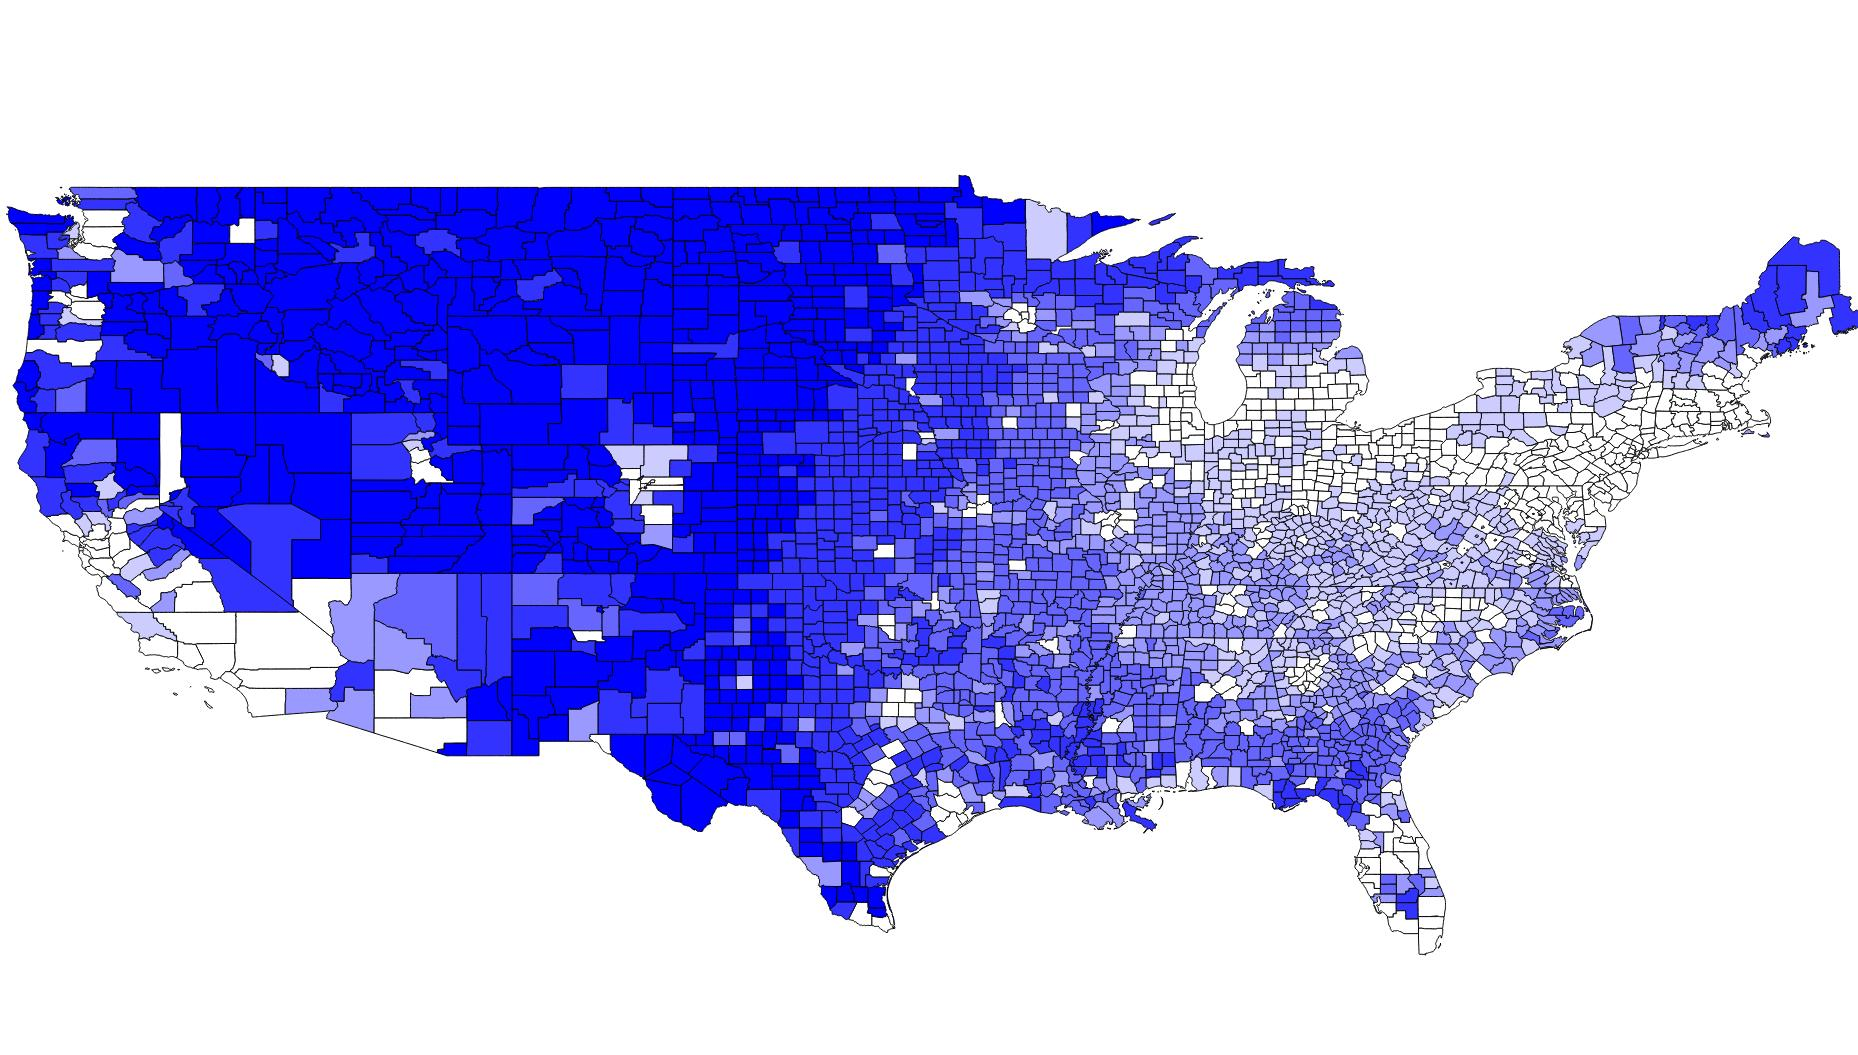
\includegraphics[width=.7\textwidth]{pics/rem.jpeg}}\quad
  \subfloat[Population]{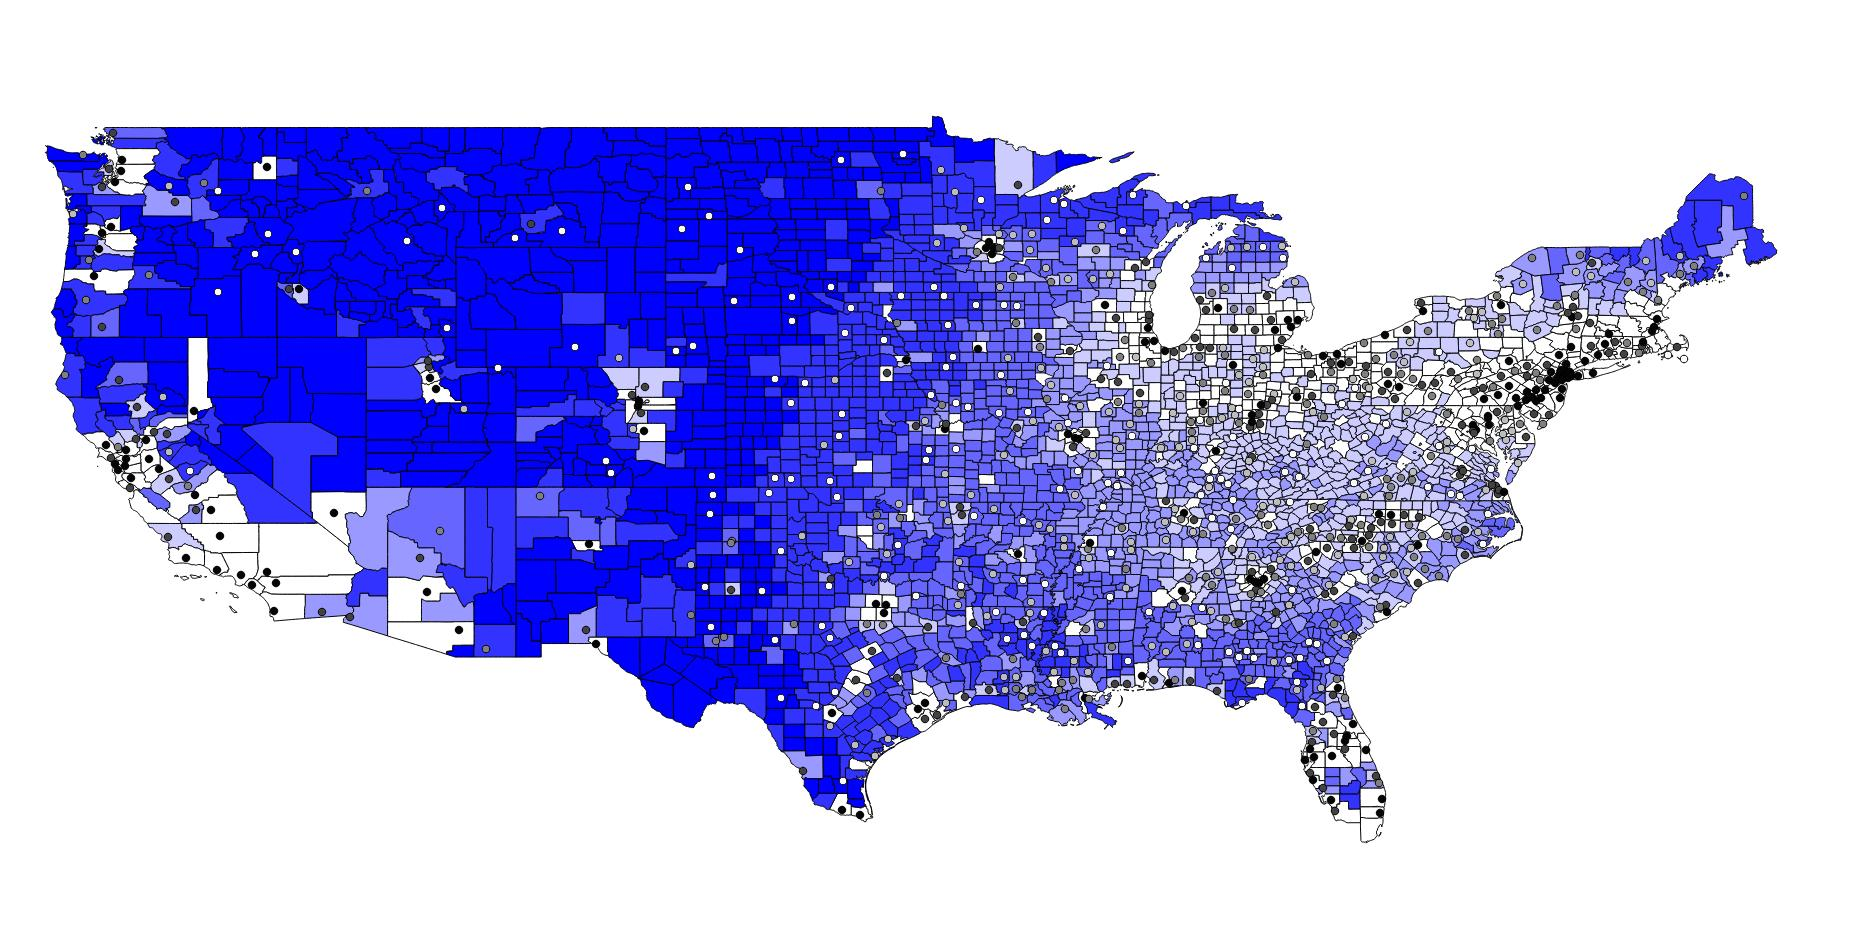
\includegraphics[width=.7\textwidth]{pics/pop.jpeg}}\\
  \subfloat[Skill Premium]{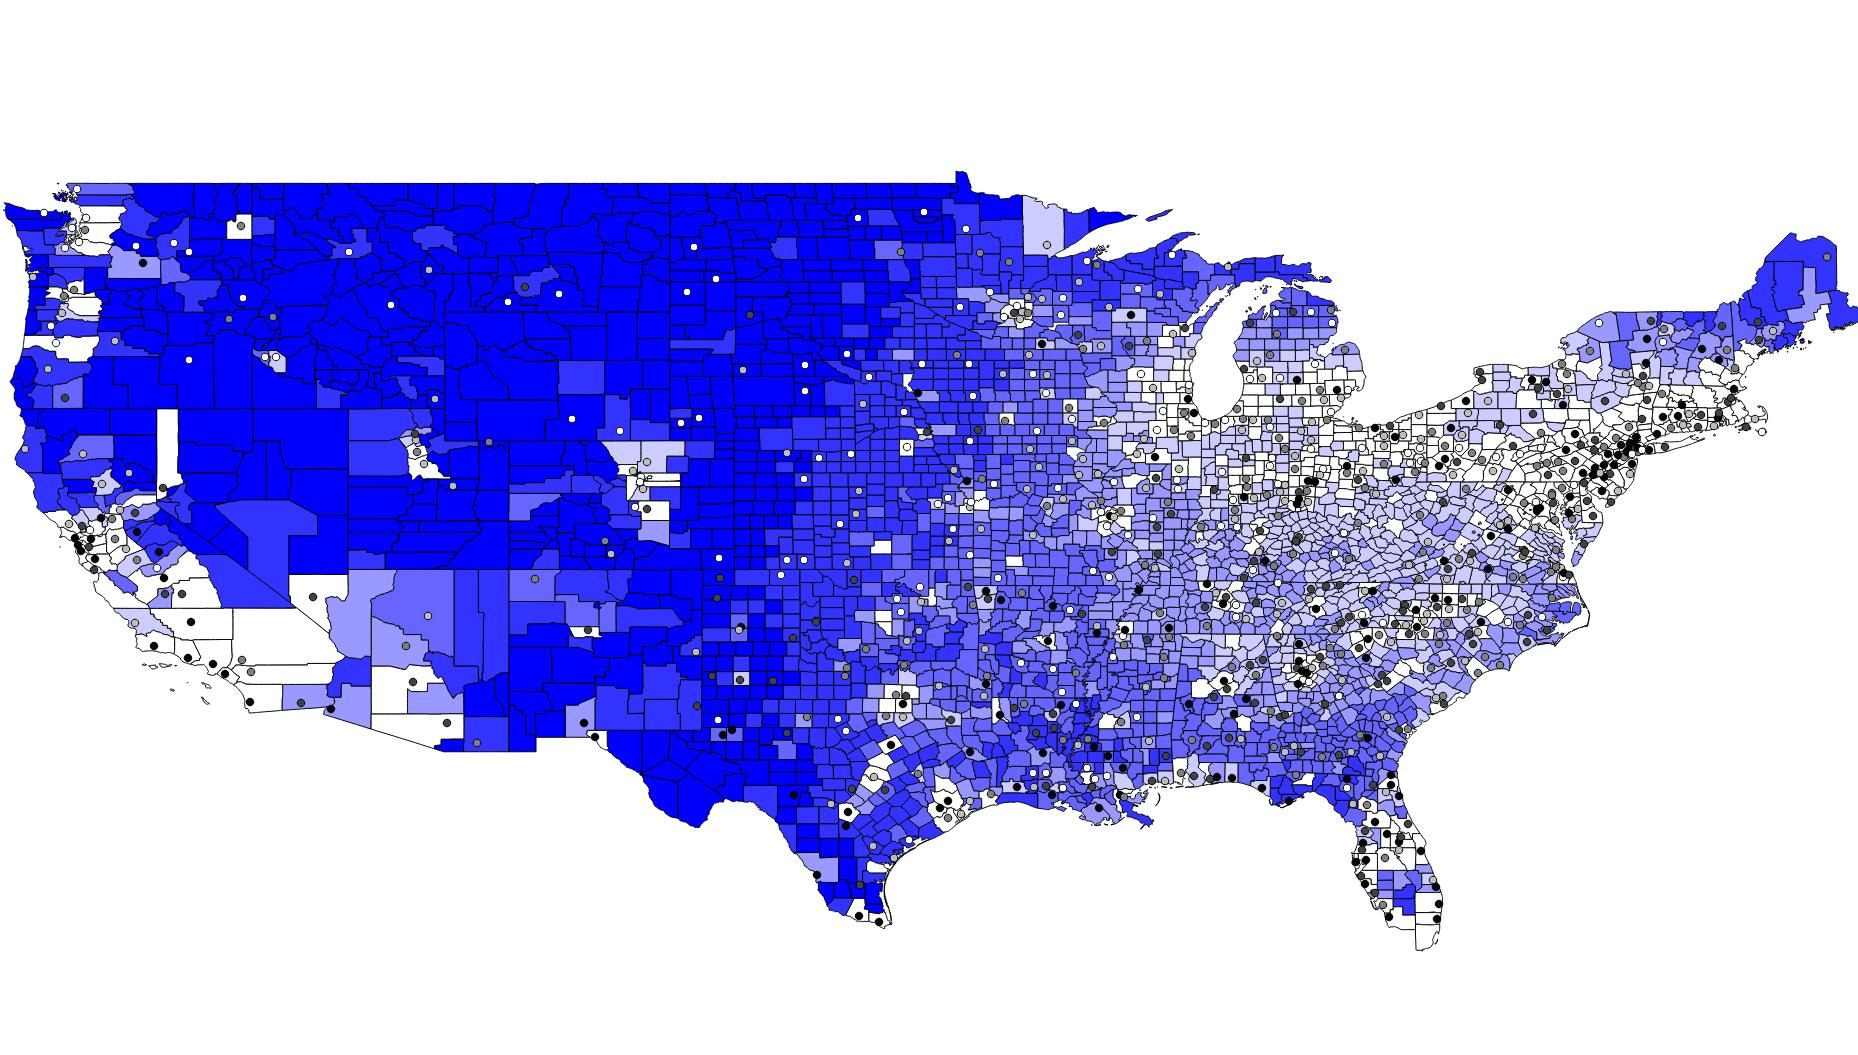
\includegraphics[width=.7\textwidth]{pics/college_wage_premium_alt.jpeg}}\quad
  \subfloat[College Share]{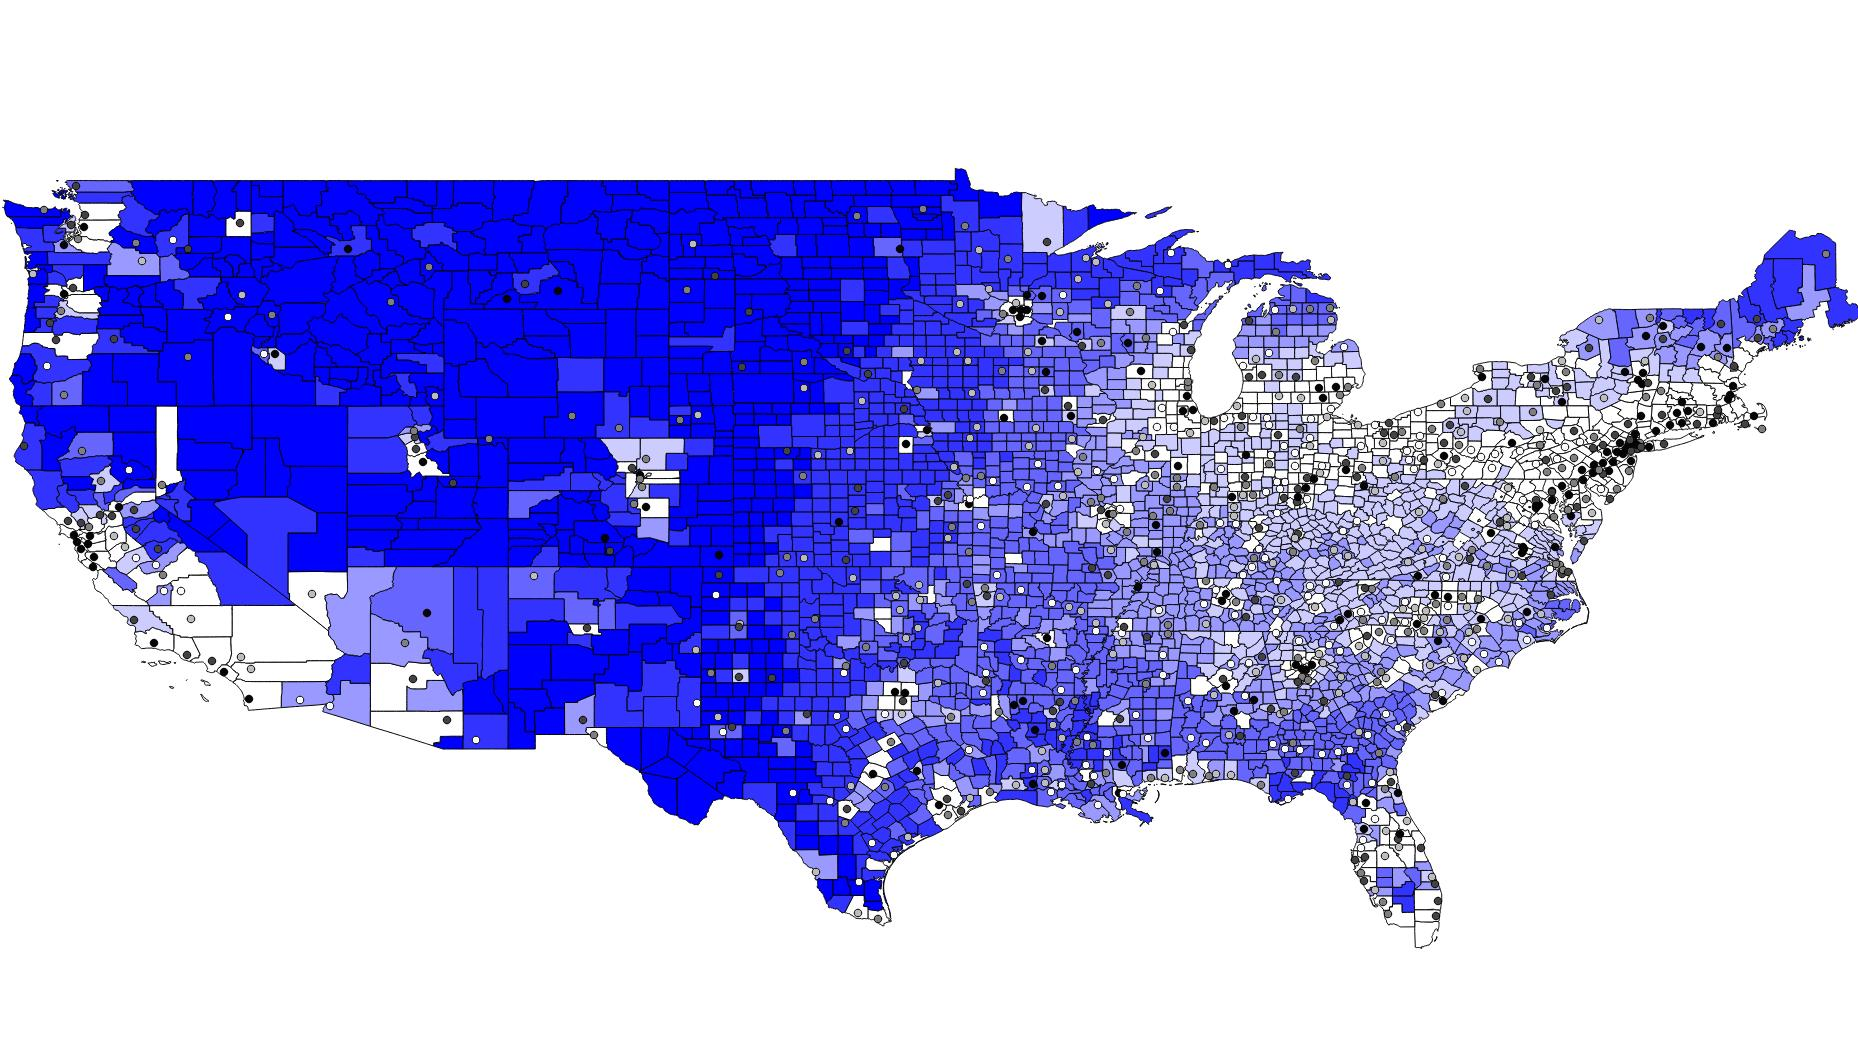
\includegraphics[width=.7\textwidth]{pics/college_pop_ratio.jpeg}}
  \caption{Counties by data feature}
  \label{fig:geo}
\end{figure}

\subsection{Empirical results}

% This table was done using estout package in stata, which is why the code looks so ugly!
\begin{table}
    \centering
    \begin{tabular}{lccc} \hline
     & (1) & (2) & (3) \\
    VARIABLES & l\_wage\_prem & l\_wage\_prem & l\_wage\_prem \\ \hline
    \vspace{4pt} & \begin{footnotesize}\end{footnotesize} & \begin{footnotesize}\end{footnotesize} & \begin{footnotesize}\end{footnotesize} \\
    l\_remote & -0.0562*** & -0.0367*** & -0.0310** \\
    \vspace{4pt} & \begin{footnotesize}(0.00558)\end{footnotesize} & \begin{footnotesize}(0.0113)\end{footnotesize} & \begin{footnotesize}(0.0125)\end{footnotesize} \\
    l\_pop &  & 0.00809** & 0.00432 \\
    \vspace{4pt} & \begin{footnotesize}\end{footnotesize} & \begin{footnotesize}(0.00391)\end{footnotesize} & \begin{footnotesize}(0.00431)\end{footnotesize} \\
    Constant & -0.275*** & -0.113 & 0.0495 \\
     & \begin{footnotesize}(0.0728)\end{footnotesize} & \begin{footnotesize}(0.112)\end{footnotesize} & \begin{footnotesize}(0.123)\end{footnotesize} \\
    \vspace{4pt} & \begin{footnotesize}\end{footnotesize} & \begin{footnotesize}\end{footnotesize} & \begin{footnotesize}\end{footnotesize} \\
    State FE & \mbox{no} & \mbox{no} & \mbox{yes} \\
    Observations & 815 & 815 & 815 \\
     $R^2$ & 0.119 & 0.124 & 0.307 \\ \hline
    \multicolumn{4}{c}{\begin{footnotesize} Robust standard errors in parentheses\end{footnotesize}} \\
    \multicolumn{4}{c}{\begin{footnotesize} *** p$<$0.01, ** p$<$0.05, * p$<$0.1\end{footnotesize}} \\
    \end{tabular}
    \caption{Regressions of log skill premium on log geography variables}
    \label{tab:skill_reg}
\end{table}


% This table was done using estout package in stata, which is why the code looks so ugly!
\begin{table}
    \centering
    \begin{tabular}{lccc} \hline
     & (1) & (2) & (3) \\
    VARIABLES & l\_pop\_share & l\_pop\_share & l\_pop\_share \\ \hline
    \vspace{4pt} & \begin{footnotesize}\end{footnotesize} & \begin{footnotesize}\end{footnotesize} & \begin{footnotesize}\end{footnotesize} \\
    l\_remote & -0.348*** & -0.182*** & -0.287*** \\
    \vspace{4pt} & \begin{footnotesize}(0.0288)\end{footnotesize} & \begin{footnotesize}(0.0536)\end{footnotesize} & \begin{footnotesize}(0.0682)\end{footnotesize} \\
    l\_pop &  & 0.0692*** & 0.0485** \\
    \vspace{4pt} & \begin{footnotesize}\end{footnotesize} & \begin{footnotesize}(0.0190)\end{footnotesize} & \begin{footnotesize}(0.0236)\end{footnotesize} \\
    Constant & -5.701*** & -4.312*** & -5.489*** \\
     & \begin{footnotesize}(0.375)\end{footnotesize} & \begin{footnotesize}(0.529)\end{footnotesize} & \begin{footnotesize}(0.675)\end{footnotesize} \\
    \vspace{4pt} & \begin{footnotesize}\end{footnotesize} & \begin{footnotesize}\end{footnotesize} & \begin{footnotesize}\end{footnotesize} \\
    State FE & \mbox{no} & \mbox{no} & \mbox{yes} \\
    Observations & 815 & 815 & 815 \\
     $R^2$ & 0.151 & 0.163 & 0.314 \\ \hline
    \multicolumn{4}{c}{\begin{footnotesize} Robust standard errors in parentheses\end{footnotesize}} \\
    \multicolumn{4}{c}{\begin{footnotesize} *** p$<$0.01, ** p$<$0.05, * p$<$0.1\end{footnotesize}} \\
    \end{tabular}
   \caption{Regressions of log college share on log geography variables}
    \label{tab:col_reg}
\end{table}

In this section we document the covariance of our measure of geography, remoteness, with our measures of inequality, the college wage premium and college share.  Regressions of the skill premium on remoteness and other variables are found in Table \ref{tab:skill_reg}.  Remoteness covaries negatively with the skill premium, with an elasticity of 5\%.  We find that the population of a county varies positively with the skill premium, a result that has been emphasized in other studies.  That the coefficient on population loses significance with state fixed effects is a provocative result.  The covariance of remoteness and the skill premium is the same order of magnitude as the covariance of remoteness with population found in the literature, but in the opposite direction.

In Table \ref{tab:col_reg} we report coefficient estimates from regressions of college population ratio on the same regressors.  We find that remoteness covaries positively with the college population ratio.  Nearly everything said about the was before, the magnitude of the population effect and the remoteness effect are similar.  The one difference is the population remains significant after including state fixed effects.

The takeaway from the empirical section is that we have identified a new relationship in the data.  Relatively remote counties in the United States have relatively low college wage premia, and relatively low college population shares.  As has been found in the previous literature we find that relatively high population counties also have relatively high college wage premia and relatively high college population shares.  These two facts motivate the theory developed in the next section.

\section{Theory}

In the last section, we presented evidence that geography plays a role in shaping the college wage premium and college population shares.  In this section we develop a theoretical model to help us understand the patterns we found: that the college wage premium and college population share both decrease with the remoteness of a location while the college share increases.

\subsection{Environment and Technology}

The model is static, with a continuum of locations $J$, a continuum of skilled workers $L_H$, and a continuum of unskilled workers $L_L$.  Workers can choose to reside and work in any (single) location.  Firms in each location can produce a location-specific variety of a tradable final good with a constant elasticity production function using the two types of labor as inputs.  There is free entry of firms in each location.  Both workers and firms are price takers.

\subsection{Worker's problem}

The utility of a worker in location $i$ is:
\begin{eqnarray}\label{eq:utility}
	Q(i) u(i) \epsilon(i)
\end{eqnarray} 
where $Q(i)$ is utility from tradeables, $u(i)$ is the utility from exogenous amenities, and $\epsilon^h(i)$ is worker $h$'s exogenous preference for location $i$.  Tradeable goods are differentiated by the origin of production, and $q(j,i)$ is consumer's cojsumption in $i$ from goods originated in location $j$. The aggregator $Q(i)$ in the utility function with elasticity of substitution $\sigma>0$ is:
\[
	Q(i) = \left[\int_J q(j,i)^{\frac{ \sigma - 1}{\sigma}}~ dj\right]^{\frac{\sigma}{\sigma-1}},
\]
We assume that worker location prefrences $\epsilon^h(i)$ are independent across workers and locations, and have a Type II Extreme Value distribution,
\[
    \Pr(\epsilon(i) \leq x) = \exp(-x^{-\theta})
\]
Workers are endowed with exogenous skill $s \in \{H,L\}$. A worker's wage in location $i$ is denoted by $w_s(i)$, and her budget constraint is 
\begin{eqnarray}\label{eq:budget}
	w_s(i) = \int_J p(j,i)q(j,i)~dj 
\end{eqnarray}
where $p(j,i)$ is price of good $j$ in destination $i$, and $J$ is the given set of locations.  The \emph{only} place skill type appears in the worker's problem, is through the wage's effect on the budget constraint.  Otherwise workers of both types have the same preferences.

An worker has two types of decision to make.  She decides where to live, and how much of each good to consume.  Given a choice of location, the second problem is standard.  A worker of type $s$ in location $i$ spends $x_s(j,i)$ on goods produced in $j$,
\begin{eqnarray}\label{eq:x_s}
	x_s(j,i) & \equiv & p(j,i) q_s(j,i) = \Big[ \frac{p(j,i)}{P(i)} \Big]^{1-\sigma} w_s
\end{eqnarray}
where $P(i)$ is the CES price index,
\begin{eqnarray}\label{eq:price_index}
	P(i) = \left[\int_J p(j,i)^{1-\sigma}~ dj\right]^{\frac{1}{1-\sigma}}
\end{eqnarray}

The second decision a worker makes is where to live.  In order to characterize this decision, we introduce congestion forces as in \citet{allen2014trade}:
\begin{eqnarray}\label{eq:congestion}
u(i) = \bar{u}(i)  n(i)^{\gamma}
\end{eqnarray}
Here, $n(i)$ is total population in location $i$ and $\gamma<0$ is the degree of congestion effect. This specification is isomorphic to a setting where preferences are Cobb-Douglas between tradeables and housing in which housing supply is inelastic.
A worker with skill level $s$ faces the following discrete choice problem over locations:
\begin{eqnarray} 
\max_{i \in J}~ \frac{w_s(i)}{P(i)}u(i) \epsilon(i)  \nonumber
\end{eqnarray}
Using the properties of the Type-II extreme value distribution, we can characterize the share of type-$s$ labor in location $i$ as:\footnote{Incidentally this equation gives the model its first testable prediction:
    \begin{equation*}
        \frac{\frac{w_H(i)}{w_L(i)}}{\frac{n_H(i)}{n_L(i)}^\frac{1}{\theta}} = \frac{\frac{w_H(j)}{w_L(j)}}{\frac{n_H(j)}{n_L(j)}^\frac{1}{\theta}}
    \end{equation*}
    A higher ratio of skilled workers to unskilled workers implies a higher skill premium in wages.}
    

\begin{eqnarray}
    \frac{n_s(i)}{n_s(j)} = \left(
	\frac{w_s(i)u(i)/P(i)}
	{w_s(j)u(j) /P(j)}\right)^\theta
    \label{eq:rel_pops}
\end{eqnarray} 
where $n_s(i)$ is population of workers with type $s$ in location $i$.
The elasticity of relative labor supply to relative wages is:
\[
\frac{ \partial \Big(n_s(i)/n_s(j)\Big) \Big/
\Big(n_s(i)/n_s(j)\Big)}
{\partial \Big(w_s(i)/w_s(j)\Big) \Big/
\Big(w_s(i)/w_s(j)\Big) } = \theta
\]
The variance of $\epsilon(i)$ across both workers and locations is decreasing in $\theta$. A large $\theta$ implies that individual unobserved preferences for location are similar across locations. Small changes in wages, prices, or amenities induce large movements of workers.  Another way of putting it is that the supply curve of workers to a location is flat.  When $\theta$ is small, workers have widely varying preferences over locations, so that large changes in wages, prices, or amenities are necessary to induce movement.  That is, the supply curve of workers to a location is steep.

There is a lot of intuition for the way the model works here already.  A location with a higher relative wage for skilled workers will attract more workers, but it won't attract all the skilled workers.  Small changes in relative wages will induce small changes in relative populations.\footnote{In a model without preference heterogeneity, in equilibrium all populated locations must offer the same utility within skill type.  This means that a location which deviates and offers a slightly higher wage will attract \emph{all} workers.}

Define the real-wage index $W_s$:
\begin{equation*}
    W_s \equiv \frac{1}{N_s}\int_{j=0}^{\|J\|}\left(w_s(j) u(j) / P(j)\right)^\theta dj
\end{equation*}
Here $N_s$ is the exogenously given total population of type-$s$ workers.  This index is a per-capita measure of welfare for workers of type $s$. Again using properties of the Type-II extreme value distribution, we derive the relationship for all $i \in J$:
\begin{eqnarray}\label{eq:indiff}
    W_s = \left(\frac{w_s(i)} {P(i)} u(i) \right)^\theta \frac{1}{n_s(i)}
\end{eqnarray}
That is, this relationship between real wages and population is constant across locations.

\subsection{Labor Demand}
Each location has a representative firm with a CES production function using skilled and undskilled workers,
\begin{eqnarray}
	 A(i)\Big[ \beta_H(i) n_H(i)^{\frac{\varepsilon-1}{\varepsilon}} + \beta_L(i) n_L(i)^{\frac{\varepsilon-1}{\varepsilon}} \Big]^{\frac{\varepsilon}{\varepsilon-1}} \nonumber
\end{eqnarray}
where $A(i)$ is total factor productivity in location $i$. $\varepsilon>0$ is the elasticity of substitution between high and low skill workers. $\beta_H(i)>0$ and $\beta_L(i)>0$ are factor intensities. In the model, differences in factor productivities (and agglomeration) are the \textit{only} things which separate skilled and unskilled labor.  Other models in the inequality literature, such as \textbf{PHD guy, who else?}, build in more fundamental differences in skilled and unskilled preferences or taste for amenities.
By cost minimization, the unit cost of production equals
\begin{eqnarray}\label{eq:unit_cost}
	 \frac{c(i)}{A(i)} ,~where~~c(i)=\Big[ \beta_H(i)^{\varepsilon} w_H(i)^{1-\varepsilon} + \beta_L(i)^{\varepsilon} w_L(i)^{1-\varepsilon}\Big]^{\frac{1}{1-\varepsilon}}
\end{eqnarray}
Share of spending of producers on high skill workers, denoted by $b(i)$, is given by
\begin{eqnarray}\label{eq:input_share}
	b(i) = \frac{\beta_H(i)^{\varepsilon} w_H(i)^{1-\varepsilon}}{\beta_H(i)^{\varepsilon} w_H(i)^{1-\varepsilon} + \beta_L(i)^{\varepsilon} w_L(i)^{1-\varepsilon}}
\end{eqnarray}
Following the literature, we distinguish two sorts of agglomeration forces. First 
\begin{eqnarray}\label{eq:agglom_general}
A(i) = \bar{A}(i) n(i)^{\alpha}
\end{eqnarray}
with $\alpha>0$. This agglomeration force changes productivity of both low and high skill workers. A Krugman type monopolistic competition generates similar force through endogenous measure of firms. In addition, there is overwhelming evidence that agglomeration forces are stronger for high skill workers\textbf{CITATION}, suggesting that high skill individuals are more productive through exchanging ideas with each other. Motivated by these findings, we let a high skill individual be more productive through concentration of high skill workers,
\begin{eqnarray}\label{eq:agglom_specific}
	\beta_H(i) & = & \bar{\beta}_H(i) n_H(i)^{\varphi} \nonumber \\
	\beta_L(i) & = & \bar{\beta}_L(i)
\end{eqnarray}

As was suggested above, the intuition for the mechanisms in the model is now available.  Larger cities will have more productive skilled workers, but unskilled workers will be exactly as productive everywhere.  Firms in relatively large cities will therefore demand a relatively high share of skilled workers.  In order to attract these workers, the location will need a relatively high skill premium.

Finally, markets are perfectly competitive. Let $d(j,i)$ be the trade costs of shipping a good from $j$ to $i$. Price of a good produced in location $j$ and consumed in location $i$, $p(j,i)$, equals $c(j)d(j,i)/A(j)$. 

\subsection{Equilibrium Definition}

A \textit{spatial equilibrium} is a set of $w_H(i)$, $w_L(i)$, $n_H(i)$, and $n_L(i)$ such that:\footnote{There is a bit hidden in this definition, as we have already used perfect competition to give us goods prices $p(j,i)$ given wages, the consumer's optimization problem to give us demand $x(j,i)$ given prices and wages, and the firm's optimization problem to give us relative labor demand \eqref{eq:input_share}}
\begin{enumerate}
\item Labor shares in locations are according to (\ref{eq:indiff}).
\item Demand and supply of skilled and unskilled labor equal in each location.
\item Goods market clear
\begin{eqnarray}\label{eq:goods_mkt_clear}
	w_H(i) n_H(i) =  b(i) \int_J \sum_{s \in \{H,L\}} n_s(i)x_s(j,i) ~dj 
\end{eqnarray}
where $x_s(j,i)$ is given by (\ref{eq:x_s}), and $b(i)$ is given by (\ref{eq:input_share}).
\item Feasible allocation of labor, $\int_J n_H(j) ~dj = N_H$ and $\int_J n_L(j) ~dj = N_L$.
\end{enumerate}

\vspace{5mm}
\subsection{Equilibrium Analysis}

Before we derive a small number of equations characterizing equilibrium, we first discuss features of the model equilibrium.  In particular, we show that without both heterogeneous location preferences as well as agglomeration forces, our model would not generate skill premia location specific skill premia in wages.  However, we need no other type of skill specific preferences or productivity to generate this result.

Perfect competition gives us that the income share of skilled labor equals firm's optimal input share on skilled labor:
\begin{eqnarray}
\frac{w_H(i) n_H(i)}{w_H(i) n_H(i) + w_L(i) n_L(i)}  = \frac{\beta_H(i)^{\varepsilon} w_H(i)^{1-\varepsilon}}{\beta_H(i)^{\varepsilon} w_H(i)^{1-\varepsilon} + \beta_L(i)^{\varepsilon} w_L(i)^{1-\varepsilon}} \nonumber
\end{eqnarray}
With some algebra, and substituting in aggomeration, we get:
\begin{eqnarray}\label{eq:labor_demand}
	\omega(i) \equiv \frac{w_H(i)}{w_L(i)} = \frac{\bar{\beta}_H(i)}{\bar{\beta}_L(i)}\Big[ \frac{n_H(i)}{n_L(i)} \Big]^{-1/\varepsilon}n_H(i)^{\varphi/\varepsilon}
\end{eqnarray}
where $\omega(i)$ is the skill premium in location $i$.

Using equation (\ref{eq:indiff}), the supply side of labor markets imply:\footnote{As far as we are aware, other models of inequality in the literature assume fundamental differences in preferences between skilled and unskilled workers.  To derive \eqref{eq:labor_supply} we are using the fact that skilled and unskilled workers face the same amenities, as well as the same prices.}
\begin{eqnarray}\label{eq:labor_supply}
    \omega(i) = \Big[\frac{W_H}{W_L} \frac{n_H(i)}{n_L(i)} \Big]^{\frac{1}{\theta}}
\end{eqnarray}
Labor markets clear when skill premia, $\{\omega(i)\}_{i \in J}$, satisfy the pairs of demand by (\ref{eq:labor_demand}) and supply by (\ref{eq:labor_supply}):
\begin{eqnarray}\label{eq:labor_demand_supply}
    n_L(i) = \left( \left(\frac{W_H}{W_L}\right)^{\frac{1}{\theta}} \frac{\bar{\beta}_L(i)}{\bar{\beta}_H(i)} \right)^{\frac{\theta \varepsilon}{ \theta+ \varepsilon}} n_H(i)^{1-\frac{\theta \varphi}{\theta+\varepsilon}}
\end{eqnarray}
The share of skilled population $n_H/n_L$ is constant across locations if skilled agglomeration is zero, $\varphi=0$. From \eqref{eq:labor_supply} we see that if the share of skilled population is constant everywhere, so is the skill premium.  Also from \eqref{eq:labor_supply}, we see that if $\theta\rightarrow \infty$ the skill premium is constant across (populated) locations.\footnote{More intuition can be gleaned from \eqref{eq:labor_demand_supply}.  If $\theta \rightarrow 0$, we see that the share of skilled population will also be constant, as no one cares about wages, only their location preference shocks which are symmetric.}  In order to have equilibria with varying skill premia, we need \emph{both} $\theta$ to be finite and $\varphi >0$.  In words, we need both variance in unobserved location preferences and the agglomeration force for skilled workers.  Large cities demand more skilled workers due to agglomeration, but when unobserved preferences matter, skilled workers do not fully adjust to a wage increase as some of them are very attached to a particular city. In this respect, our model departs from a standard Rosen-Roback (or Allen-Arkolakis) model by highlighting the interaction of agglomeration and the labor supply elasticity. 

% Define $\rho_H(i) = n_H(i)/N_H$ as the density of high skill labor. Equation (\ref{eq:labor_demand_supply}) and $ N_L = \int_J n_L(i)~di $ pin down $W_H/W_L$ only as a function of $\rho_H(i)$,
% %\begin{eqnarray}
% %\frac{W_H}{W_L} =
% %\Big(N_L\Big)^{(1+\theta \varepsilon)/\varepsilon}\Bigg[ \int_J \Big(  \frac{\bar{\beta}_H(i)}{\bar{\beta}_L(i)} \Big)^{-\varepsilon/(1+\theta \varepsilon)} \Big( n_H(i) \Big)^{1-\varphi/(1+\theta \varepsilon)}~di \Bigg]^{-(1+\theta \varepsilon)/\varepsilon}
% %\end{eqnarray}
% \begin{eqnarray}\label{eq:WHtoL}
% \frac{W_H}{W_L} =
% \underbrace{\Big(N_H/N_L\Big)^{-(\theta+ \varepsilon)/\theta\varepsilon}}_{\mbox{scarcity}} \times \underbrace{N_H^{\varphi/\varepsilon}}_{\mbox{agglom.}} 
% \times
% \underbrace{\Bigg[ \int_J \Big( \frac{\bar{\beta}_H(i)}{\bar{\beta}_L(i)} \Big)^{-\theta\varepsilon/(\theta+\varepsilon)} \Big( \rho_H(i) \Big)^{(\theta(1-\varphi)+\varepsilon)/(\theta+\varepsilon)}~di \Bigg]^{-(\theta+ \varepsilon)/\theta\varepsilon}}_{\mbox{allocation}} 
% \end{eqnarray}
% Equation (\ref{eq:WHtoL}) decomposes the three forces behind real well-being inequality of marginal workers: 1) Aggregate scarcity of high skill labor, 2) Aggregate agglomeration advantage of high skill workers, 3) A weighted average of relative productivities in which weights are the density of high skill labor. While the  first two behave at the aggregate, the third relates to the distribution of population. In addition, note that agglomeration is less effective when the elasticity of substitution between high and low skill labor, $\varepsilon$, is higher.

\subsection{Equilibrium equations}

In this section we characterize our equilibrium with only two integral equations.  These integral equations will be the basis of our empirical exercise.  

By simply inverting the definition \eqref{eq:input_share} of input share $b(i)$, we get total income in $i$ equal to $\frac{1}{b(i)} w_H(i)n_H(i)$. Using the goods market clearing condition, equation (\ref{eq:goods_mkt_clear}), we derive: 
\begin{eqnarray}
	w_H(i) n_H(i) b(i)^{-1} = 
	\int_J \Big[ \frac{c(i) d(i,j)}{A(i) P(j)} \Big]^{1-\sigma} w_H(j) n_H(j) b(j)^{-1} ~dj \nonumber
\end{eqnarray}

Equations (\ref{eq:unit_cost}) and (\ref{eq:input_share}) further imply that 
\begin{eqnarray}\label{eq:ctilde}
	c(i) & = & \tilde{c}(i) w_H(i) \nonumber \\
    \mbox{where}~~~ \tilde{c}(i) & = & 
	\Big[\bar{\beta}_H(i) n_H(i)^{\varphi}\Big] ^{\frac{\varepsilon}{1-\varepsilon}} \Big[b(i)\Big]^{\frac{-1}{1-\varepsilon}}
\end{eqnarray}
Replacing $c(i)$ with $\tilde{c}(i)$ in the above integral equation and also replacing the price index using (\ref{eq:indiff}), after some algebra we get:
\begin{eqnarray}\label{eq:system1}
	& & A(i)^{1-\sigma} \tilde{c}(i)^{\sigma-1} n_H(i)  w_H(i)^{\sigma}  b(i)^{-1}  \nonumber \\
	& & =  
    W_H^{\frac{1-\sigma}{\theta}}
	\int_J d(i,j)^{1-\sigma} u(j)^{\sigma-1} n_H(j)^{(\theta+1-\sigma)/\theta} w_H(j)^{\sigma} b(j)^{-1}  ~dj
\end{eqnarray}
Again substituting the price index from (\ref{eq:indiff}) and $\tilde{c}(i)$ into (\ref{eq:price_index}), we get another integral equation: 
\begin{eqnarray}\label{eq:system2}
 	& &  u(i)^{1-\sigma} n_H(i)^{(\sigma-1)/\theta} w_H(i)^{1-\sigma}  = \nonumber \\ 
 	& & 
    W_H^{\frac{1-\sigma}{\theta}}
 	\int_J  d(j,i)^{1-\sigma} A(j)^{\sigma-1}  \tilde{c}(j)^{1-\sigma} w_H(j)^{1-\sigma}
 	~ dj
\end{eqnarray}
Equations \ref{eq:system1}--\ref{eq:system2} give us two systems of integral equations. If $\varphi=0$ and $\theta=\infty$, the integral equations collapse to those in \citet{allen2014trade}. 

We can reduce our system further using a trick from \citet{allen2014trade}.  If either of the systems of integral equation hold allong with the following relation, both systems of integral equations must hold:
\begin{eqnarray}\label{eq:systems_relation}
	\frac{w_H(i)^{\sigma}n_H(i)A(i)^{1-\sigma}\tilde{c}(i)^{\sigma-1}}{b(i)} = \lambda w_H(i)^{1-\sigma} u(i)^{1-\sigma} n_H(i)^{(\sigma-1)/\theta}
\end{eqnarray}
where $\lambda > 0$ is some constant.

\subsection{Solution Algorithm}

\begin{enumerate}
\item Guess $n_H(i)$ for all $i$.
\item Compute $W_H/W_L$ according to (\ref{eq:WHtoL}). Then plug it in (\ref{eq:labor_demand_supply}) to find $n_L(i)$.
\item Calculate skill premia, $\omega(i)$, according to (\ref{eq:labor_supply}).
\item Compute $b(i)
= 1/(1 + \frac{n_L(i)}{n_H(i)} \frac{1}{\omega(i)})$
\item Find $\tilde{c}(i)$ according to (\ref{eq:ctilde}).
\item Calculate $w_H(i)$ according to (\ref{eq:systems_relation}) (up to a scale imposed by $\lambda$)
\item Let $f(i)=w_H(i)^{1-\sigma}$, $\kappa=W_H^{1-\sigma}$, and
\[
K(j,i) = n_H(i)^{(1-\sigma)/\theta}u(i)^{\sigma-1} d(j,i)^{1-\sigma} A(j)^{\sigma-1} \tilde{c}(j)^{1-\sigma}
\]
Then, rewrite (\ref{eq:system2}) as follows:
\[
f(i) = \kappa \int_J K(j,i) f(j)~dj
\]
In iteration $t$, update $f^{(t)}(i)$ according to
\begin{eqnarray}
	f^{(t+1)}(i) = \frac{\int_J K(j,i) f^{(t)}(j)~dj}{\int_J \int_J K(j,i) f^{(t)}(j)~dj di}
\end{eqnarray}
\item Find $\lambda$ such that $N_H=\int_J n_H(i)~di$.
\end{enumerate}

\newpage

\bibliographystyle{apa.bst}
\bibliography{/home/veryshuai/Documents/research/bib/biglist}

\end{document}
